%!TEX root = ../master.tex
\chapter{Design}\label{ch:design}
\todo{This part needs rework. Write after chapter is done.}
This chapter will cover the design iterations and the decisions that were made. 

\section{Initial brainstorm}\label{sec:initialbrainstorm}
The initial brainstorm consisted of two brainstorms that was chained together. The starting point of the first brainstorm was the point 'Image to sound' and the second brainstorms starting point was 'Filters', which both are highlighted in orange. Within the 'Image to sound' brainstorm the topics that was picked were coloured blue. Where the topics chosen in the 'Filters' were coloured in red. 

\begin{figure}[!h] 
\centering
\includegraphics[width=1\textwidth]{initialbrainstorm}
\caption{\label{fig:initialbrainstorm} The initial brainstorm.}
\end{figure}

All the points from 'Image to sound' are a mixture of manipulative image processing factors and image capturing methods. 
The points expanding from 'Filters' relates to tools the user can apply to the audio created from the image. 
'Filters' branches out to the point called 'Different Filters' which lists various common filters that may be applied to the audio. It also branches out to the point called 'Controls' which allows the control of the different coefficients in filters and therefore the output of a filter. 
Since it is stated in the final problem statement that it is a requirement to be able to control the filters, the point 'Controls' is essential in the brainstorm. From 'Controls', different methods of controlling filters were considered, and from these 'Toggle all filters', 'Intensity of filter', 'Multiple filters at once' and 'Peripheral devices to adjust intensity' were chosen for the design.

Based on the final problem statement, the design team chose to narrow down the brainstorm, which resulted in working with an RGB image that can be replaced at any time. Then bandpass, comb and high shelf filters are applied, and the user is able to apply these individually or at the same time with the possibility to change the intensity of the filters by using peripheral devices. 
The reason for choosing the specific filters is the theory behind them. Many of the listed filters are similar in the way they work, but the chosen filters differentiate between each other in the way they alter the sound.


\section{Conceptual model}\label{sec:conceptualmodel}
This project will work with audiolisation of an image. The initial design is focused on the conversion of images into an audio signal. Each pixel has a value for each RGB colour channel that can be converted into a range that fits the human hearing, which is defined to be between 20 to 20.000Hz \cite{Dsp1997}. The output of this operation can then be manipulated by audio processing filters. The concept includes a control interface in the artefact. It allows the user to have control over the output in real time, as the control interface will change how the filter effects will modify the image-created audio. This gives the user agency of how the output will sound. To allow the user to create even more unique sounds, multiple filter can be applied simultaneously. This allows for a wide range of artistic expression, as the user will have control over the audio output.


\section{Peripheral devices}\label{sec:periphealdevices}
The user has to be able to affect the audio the image generates by interacting with a physical interface. The system will apply an effect which can be modified through a physical device which changes the variable range of the power of the effect from 0\% to 100\%, or in numbers 0 to 1. For this interface these different variations of a peripheral devices has been considered: 

\begin{itemize}
\item Button
\item Pressure sensor
\item Ultra sonic distance sensor
\item Potentiometer
\item Slider
\item Bend sensor
\end{itemize}

Each of these peripheral devices makes the user interact with the prototype differently and changes the functionality of the prototype depending on which peripheral device are implemented. Several conjectures can be made regarding the usability and appropriateness of each peripheral device. The peripheral device controls some sort of graduation in two directions. 

The button's functionality is it can be clicked. The button have two states: low and high. The low state is when the button is not clicked, and the high state is when the button is being clicked. This means that a system using a button will have programmed states, which will be cycled through in a predetermined or random direction. In the case that the button (telegraph or otherwise) is used to increase or decrease a given effect in steps, it presents a lack user control for fine adjustments. Furthermore, if the user wishes to quickly move from one end of the spectrum to the other one button must be pressed repeatedly which can be straining.

Variable resistors allow a system to have a position between the two extremes of low and high. This allows the system to have more fluent control than a simple binary choice of on or off. There are multiple variable resistors to choose from, which changes the user's interaction with the given device depending on the used peripheral device.  They all function in a fundamentally similar way. The question that remains is then which is more usable in our context. This can be evaluated using the notions of perceived affordance, feedforward, and feedback as defined by Norman \cite{Norman:1999:ACD:301153.301168}.

Pressure sensors react to being pressured, such as from touching and pushing. More pressure equals to a higher position on the scale. The pressure sensor affords pushing, however, it does not provide any feedforward regarding the fact that it is a pressure sensor. This means that any information the user receives from feedback, that could potentially enlighten them with this fact is from the software or a label. Disregarding that hurdle, the user receives feedback from the sensation of pressure they apply to the sensor. 

Ultra sonic distance sensors measures the distance between the sensor and a surface in front of the sensor by sending out pulses. The further away the sensor is from an object, the more frequent it will send out a pulse until the echo returns to the sensor. The distance sensor provides neither perceived affordance, feedforward or feedback on its own in any way, however, an exception can be made in its case, depending on the context of use. In an art gallery for instance, the device can potentially make the system provide incidental feedback, since potential users that simply walk by the installation will modulate the sound. This, from the users' perspective, unexpected behaviour invites curiosity. Thus it is worth considering as a peripheral device, even if it does not perform well in a formal evaluation of affordance, feedforward, and feedback.

Potentiometers can adjust between a minimum and maximum position. Depending on how much the potentiometer is turned it will result in the scale output from the device. Turning knobs is an example of potentiometers. A slider is a variant of a potentiometer with a linear interface instead of a rotary one. Through an affordance lens it becomes clear that the potentiometers the make use a turning knob are a problematic choice. The potentiometers that make use of grooves for better gripping provide the affordance that they can be turned, but it does not indicate whether turning it one way or the other affects the system in a certain way. Furthermore, it provides no feedback as to the state of the module. The slide potentiometer, when labeled with a minimum and maximum, performs much better in this respect. It clearly and intuitively provides the affordance, that force can be applied to the slider to move it, and that this controls some sort of position on a scale. The slider also provides feedback with its position in the potentiometer in that it directly corresponds to a position on the scale it controls. 


Unlike the previously mentioned variable resistors that all have a clear low and high state, the bend sensor functions differently. The bend sensor rests at a mid-point between low and high. Depending on which direction the sensor is bent the resistance will either go up or down.

Any of these devices is used as a variable controller for the different effects. Depending on which device is chosen, the integration for the user will be different. This will be tested in the iterations of the prototype and discussed further to make sure that the interface is user-friendly and easy to understand. 

\section{Electrical Component Test}\label{sec:comptest}
To figure out which electrical components the users prefers and think is the most intuitive to use, an electrical component test was conducted. All the previous mentioned electronic components were used in the test, though there was two different buttons and 3 different potentiometers. All the different components can can be seen on Figure \ref{fig:komponenter}. These components were all mounted on a cardboard plate as seen on Figure \ref{fig:componenttest}.

\begin{figure}[!h] 
\centering
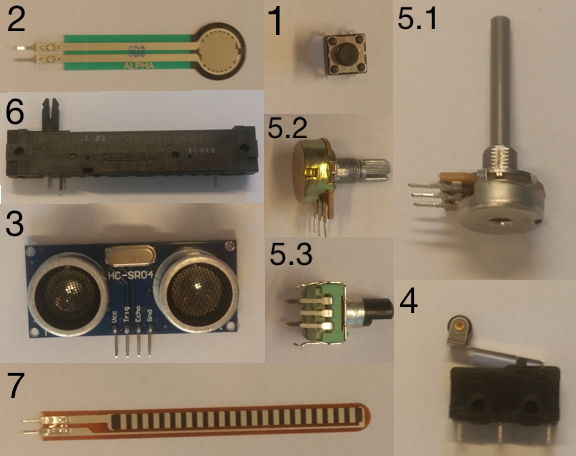
\includegraphics[width=1\textwidth]{komponenter}
\caption{\label{fig:komponenter} The 9 different components used in the test: 1. Normal push button, 2. Pressure sensor, 3. Ultrasonic distance sensor, Telegraph button, 5.1, 5.2, and 5.3 are the different potentiometers, 7. Bend sensor.}
\end{figure}

\begin{figure}[!h] 
\centering
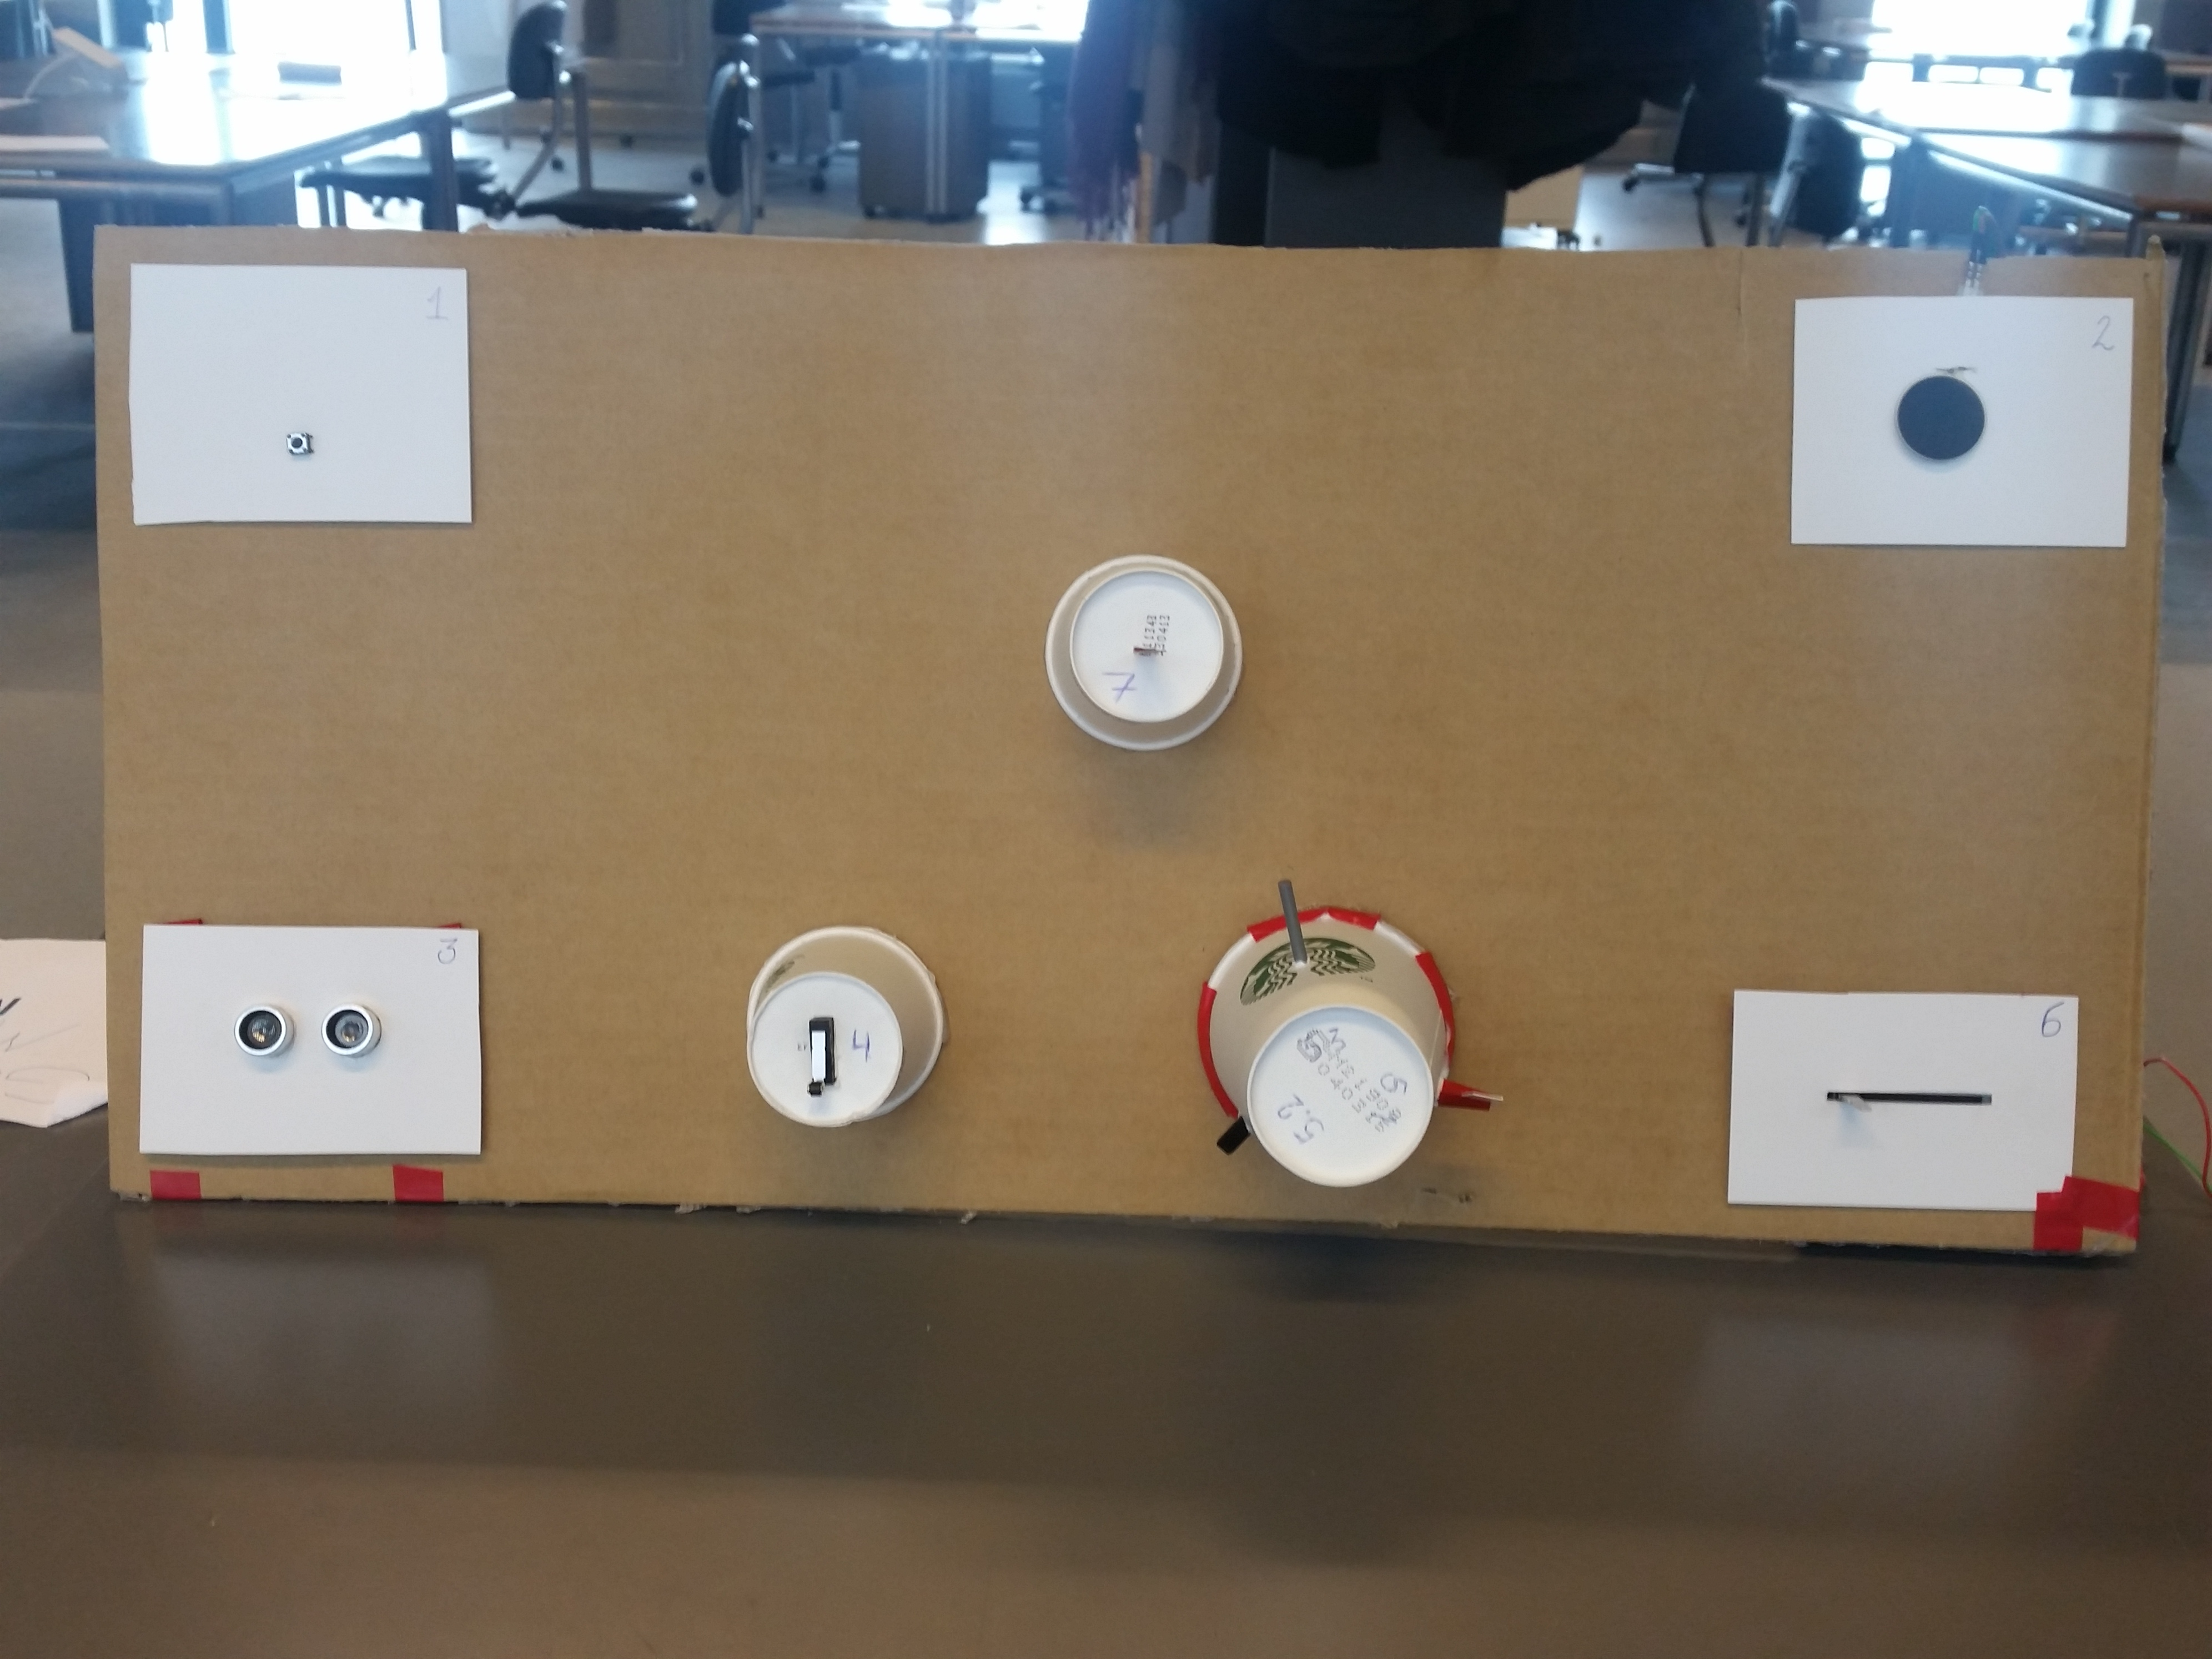
\includegraphics[width=1\textwidth]{componenttest}
\caption{\label{fig:componenttest} The component board used in the component test used to determine which electrical component to use.}
\end{figure}

The test was conducted on 10 participants, all fellow students from Medialogy. The participants were explained by 'Test Facilitator 1' how each component worked and how to interact with them. They were told that they had to use all of the components one at a time in a numeral order and think out loud when using the components. 'Test Facilitator 2' turned the volume of the music up and down, all depending on how the participant used the component.
Results, as can be seen on Table \ref{tab:electritest}, showed the participants preferred using the slider when changing the volume of the music. Based on this result and the evaluation made in Section \ref{sec:periphealdevices} a new design was created.

\begin{table}[!h]
\centering
\caption{Results of the electrical component test.}
\label{tab:electritest}
\begin{tabular}{|l|c|c|c|c|c|c|c|c|c|}
\hline
Electrical Component & 1 & 2 & 3 & 4 & 5.1 & 5.2 & 5.3 & 6 & 7 \\ \hline
Amount of votes & 1 & 0 & 3 & 0 & 0 & 0 & 0 & 6 & 0 \\ \hline
\end{tabular}
\end{table}


\section{The chosen sketch}\label{sec:thechosensketch}
Based on feedback from the components test, an interface design sketch were made to make a paper mock-up test, the sketch can be seen on Figure \ref{fig:sketchmock}. 

\begin{figure}[!h] 
\centering
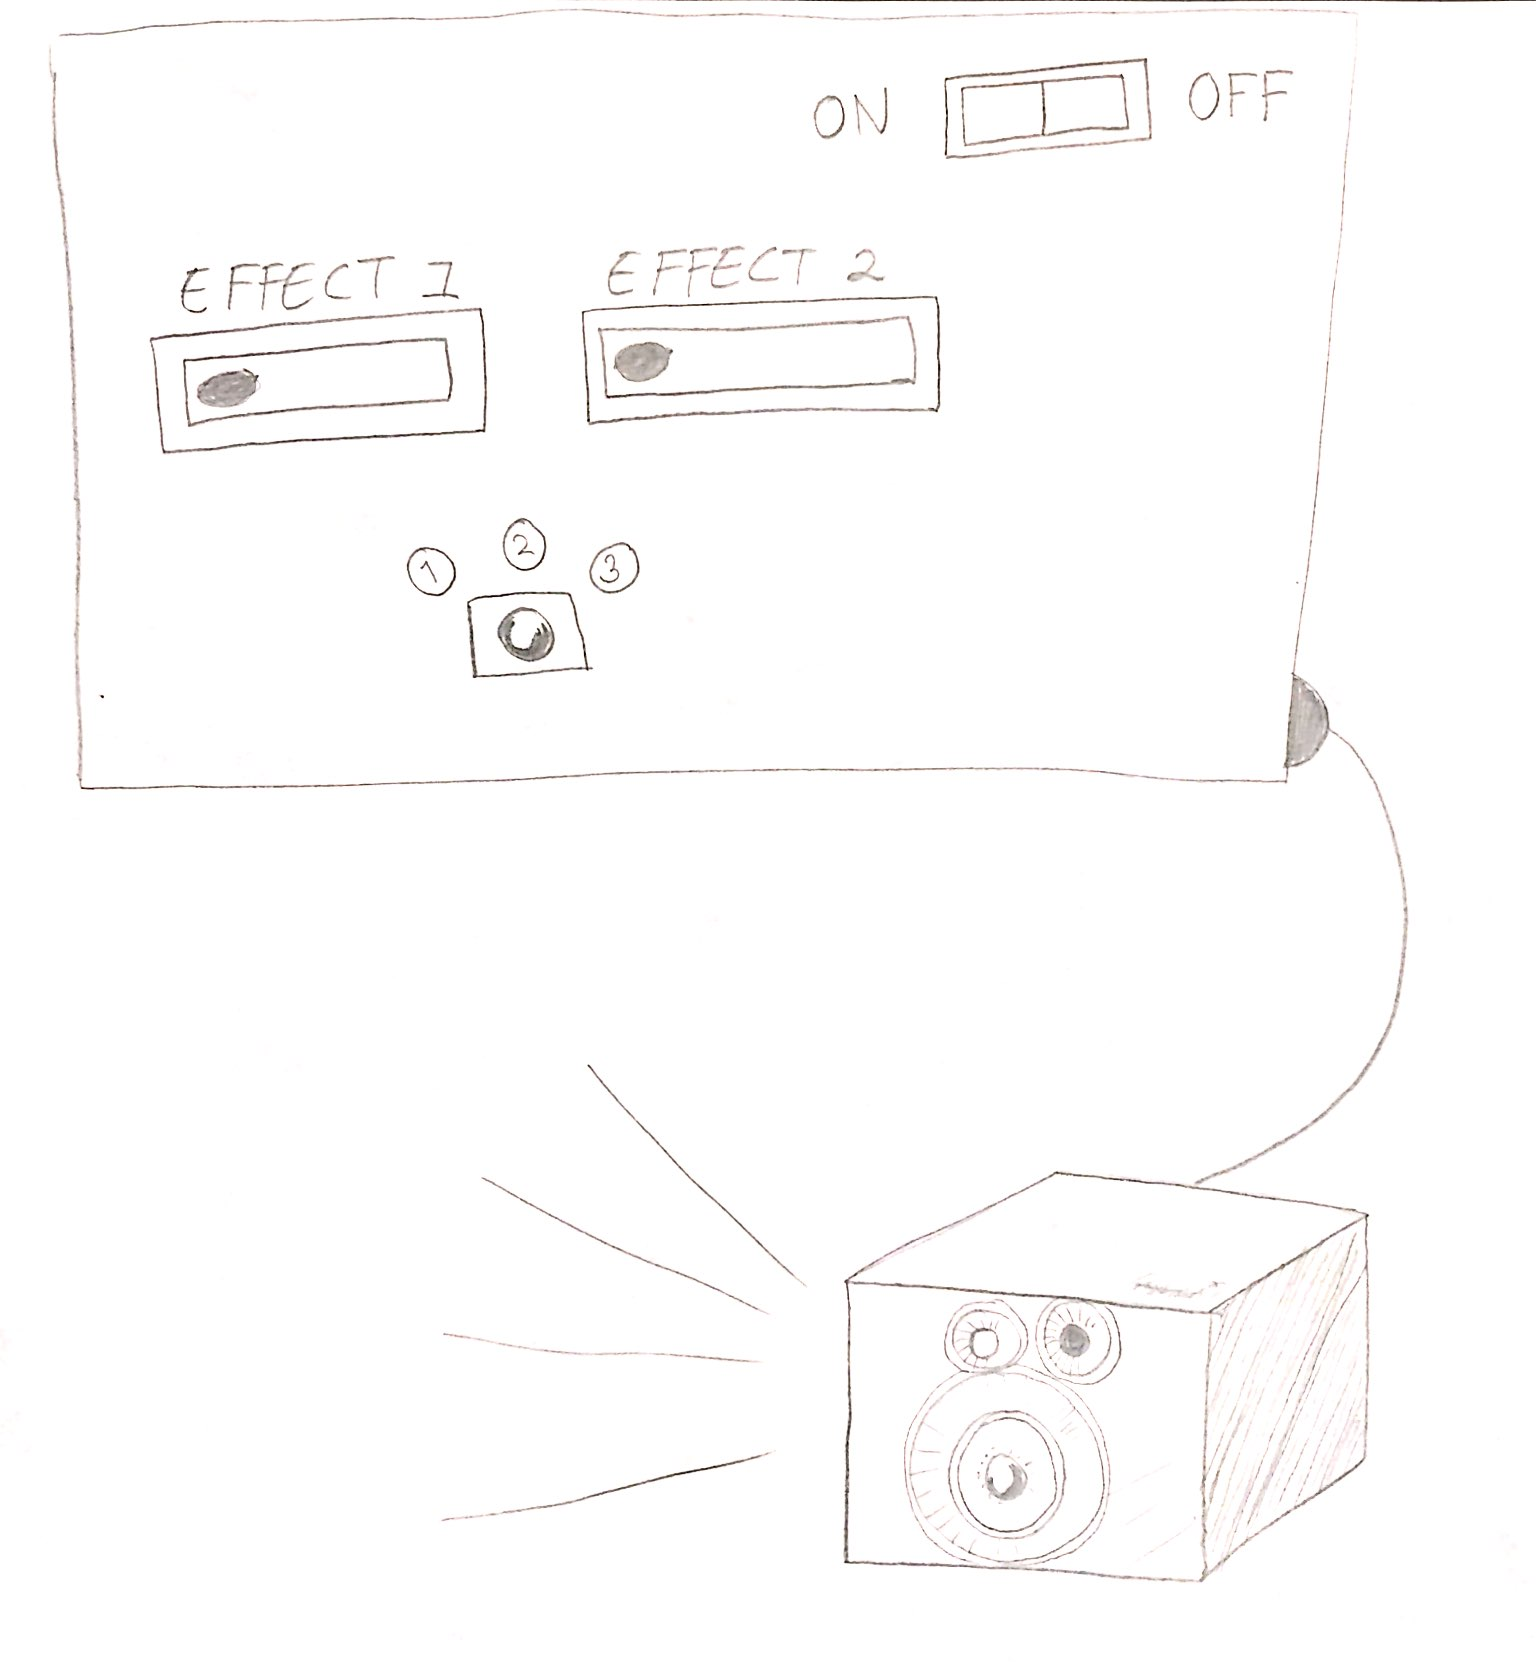
\includegraphics[width=1\textwidth]{sketchmock}
\caption{\label{fig:sketchmock} Sketch showing the chosen interface for a paper mock-up test.}
\end{figure}

The chosen sketch consists of an on/off button, two sliders with two different effects and a button that changes the state of the effects. When the device is turned on it automatically goes into state one which turns on 'Effect 1'. When the user presses the button, the device switches to state two, which turns off 'Effect 1' and turns on 'Effect 2'. When pressed for the second time, the device goes into state three where both 'Effect 1' and 'Effect 2' is turned on simultaneously. If pressed again, the circuit goes back to state one. Slider one (the left one) controls the intensity of 'Effect 1' and is only active in state one and three. Slider two (the right one) also controls the intensity but for 'Effect 2' and is active under state two and three.

\section{Interface low-fi test}\label{sec:lowfitest}
The chosen sketch was made into a paper mock-up to test the percieved affordance and the feedforward. Since it was a paper mock-up, no electronic components were used. What should have been the audio feedback was replaced with an drawing of a light bulb in order for understanding the intention of changing the intensity of an object. The paper mock-up can be seen on Figure \ref{fig:Papermockoff}.

\begin{figure}[!h] 
\centering
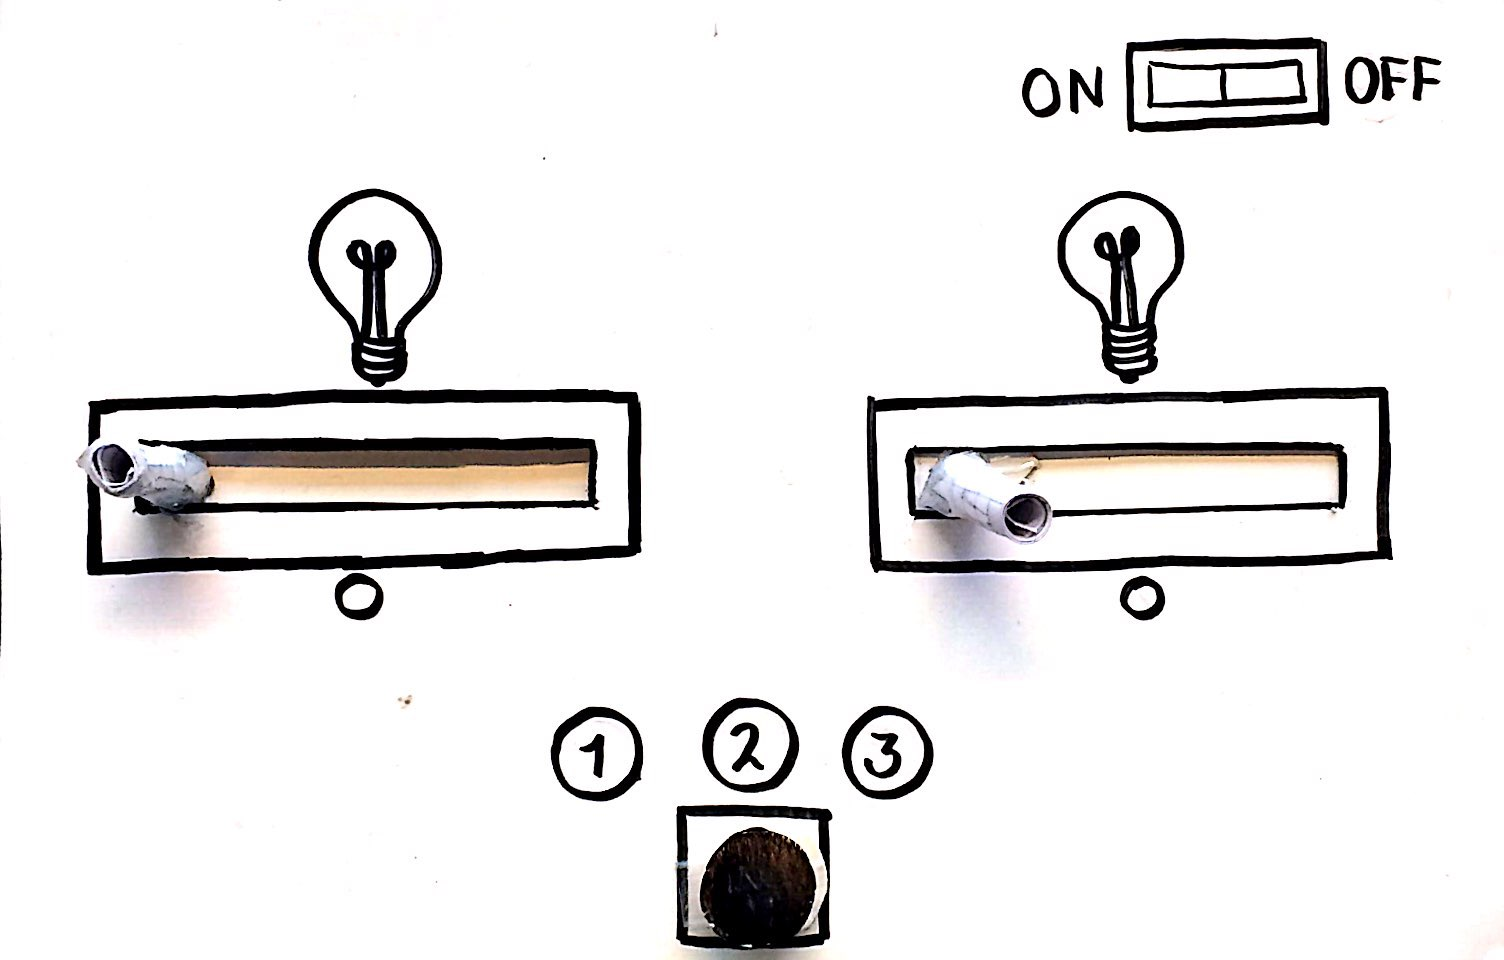
\includegraphics[width=1\textwidth]{Papermockoff}
\caption{\label{fig:Papermockoff} shows the low-fi paper mock-up of interface.}
\end{figure}

The mock-up was tested on 6 fellow Medialogy students. 'Test Facilitator 1' explained how the interface works and asked the participant to execute the following tasks:

\begin{itemize}
\item Turn on the device
\item Turn on slider 1
\item Change the intensity of the illumination of light bulb 1
\item Turn on slider 2
\item Change the intensity of the illumination of light bulb 2
\item Turn on both sliders
\item Change the intensity of both or individually both light bulbs
\item Turn off the device
\end{itemize}

Results showed that it was clear that to the user that he/she had to use the slider to change the intensity of the light bulb. However, switching between the states of which slider was in use, proved to be difficult for the user since their perception the feedforward was not clear enough. Some users suggested the use of imagery for better understanding of the interface. Since the feedforward of the slider was not sufficient enough, a feedforward test was conducted.

\section{Feedforward test}\label{sec:fftest}
Eight different designs for the slider was made, as can be seen on the Figure \ref{fig:fftestimage}.

\begin{figure}[!h] 
\centering
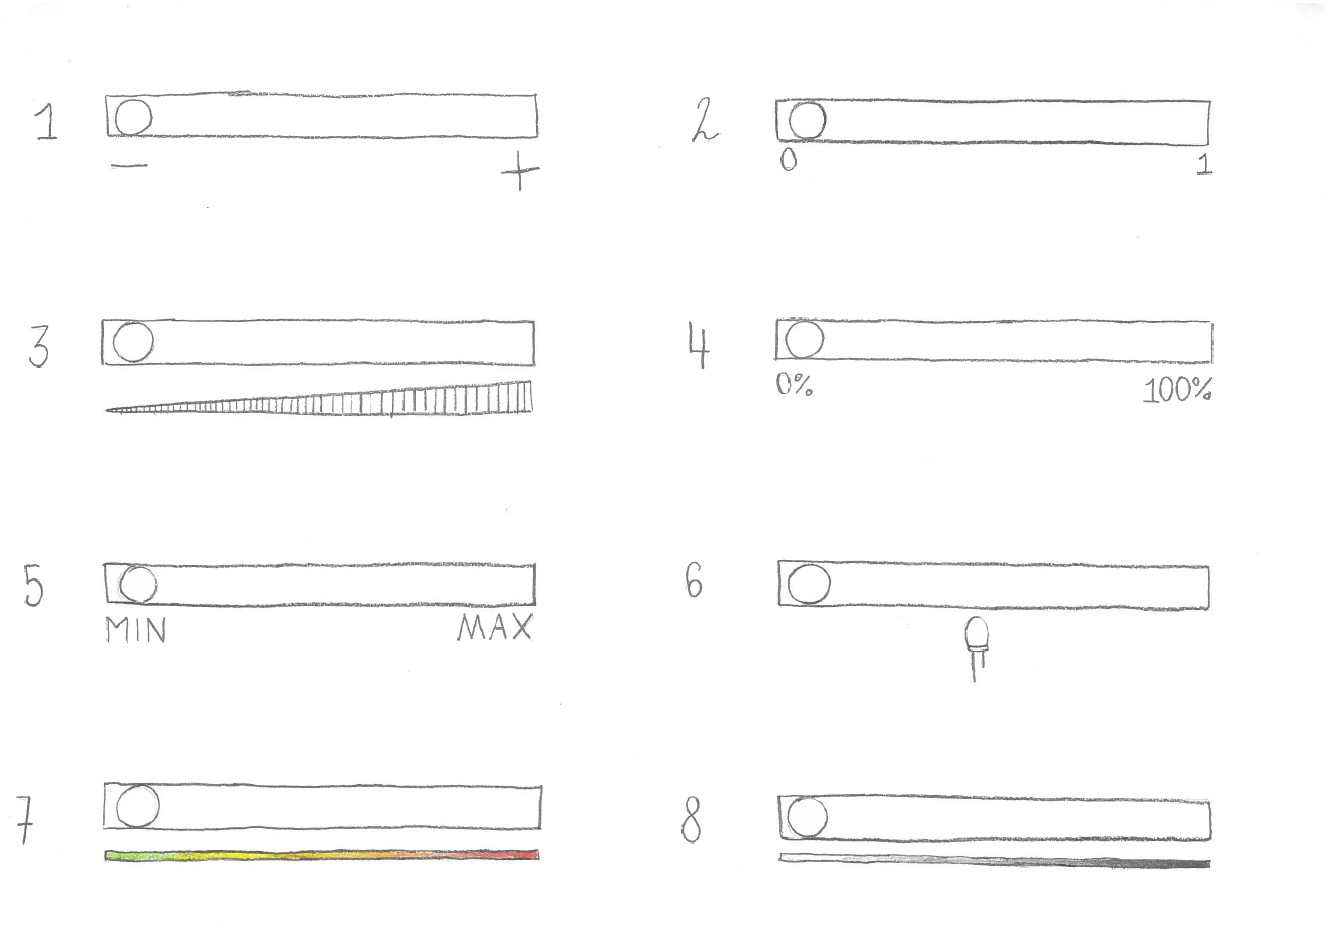
\includegraphics[width=1\textwidth]{fftestimage}
\caption{\label{fig:fftestimage} The 8 different designs for the feedforward test.}
\end{figure}

The participants for this test were also from the Medialogy studies. The test included 46 participants. The test facilitators explained the context of use for the slider and after asked the participants to choose one of the eight different designs that they thought had the best feedforward. The participants were all sitting in their group areas, so to ensure the participants answers were not affect each others, they were asked to point at a piece of paper with numbers, representing the different designs, randomly located on the paper to further ensure confidentiality when telling the test facilitator what their answers were. 

\begin{table}[!h]
\centering
\caption{Shows the results of the feedforward test.\label{tab:sliderresults}}
\begin{tabular}{|l|c|c|c|c|c|c|c|c|}
\hline
Design & 1 & 2 & 3 & 4 & 5 & 6 & 7 & 8 \\ \hline
Amount of votes & 2 & 2 & 14 & 9 & 15 & 1 & 3 & 0 \\ \hline
\end{tabular}
\end{table}

Statistically speaking, the most preferred feedforward was design five which had 15 votes, while design three received 14 votes and design four had 9 votes.
Even though design three and design five received almost the same amount of votes, the design team choose to go with the fifth design. The prototype will be expanded of this design and it will be taken into further iterations of the performance testing. 

\section{Storyboard}\label{sec:storyboard}
<<<<<<< HEAD
The picture shown in \ref{fig:Flowdiagram} shows a narrative story board, explaining how the product could be used in context. The setting of the story board is at an art museum. The user is a visitor at the museum, he walks by a large picture of a woman, in front of the picture is a box with sliders in top ( the final product \ref{fig:finalinterfacesketch3grey} ) and speakers above the picture. The user reads the description placed on the box and starts to manipulate with the sliders. The result is a user made sound coming of the speakers, and the user is happy with his creation. 
=======
The picture shown in \ref{fig:Flowdiagram} shows a narrative story board, explaining how the product could potentially be used in context. The setting of the story board is at an art museum. The user is a visitor at the museum, he walks by a large picture of a woman, speakers beside the picture and a box with sliders. The user reads the description placed on the box and starts to manipulate with the sliders. The result is a user made sound coming of the speakers, and the user is happy with his creation. 
>>>>>>> origin/master

\begin{figure}[!h] 
\centering
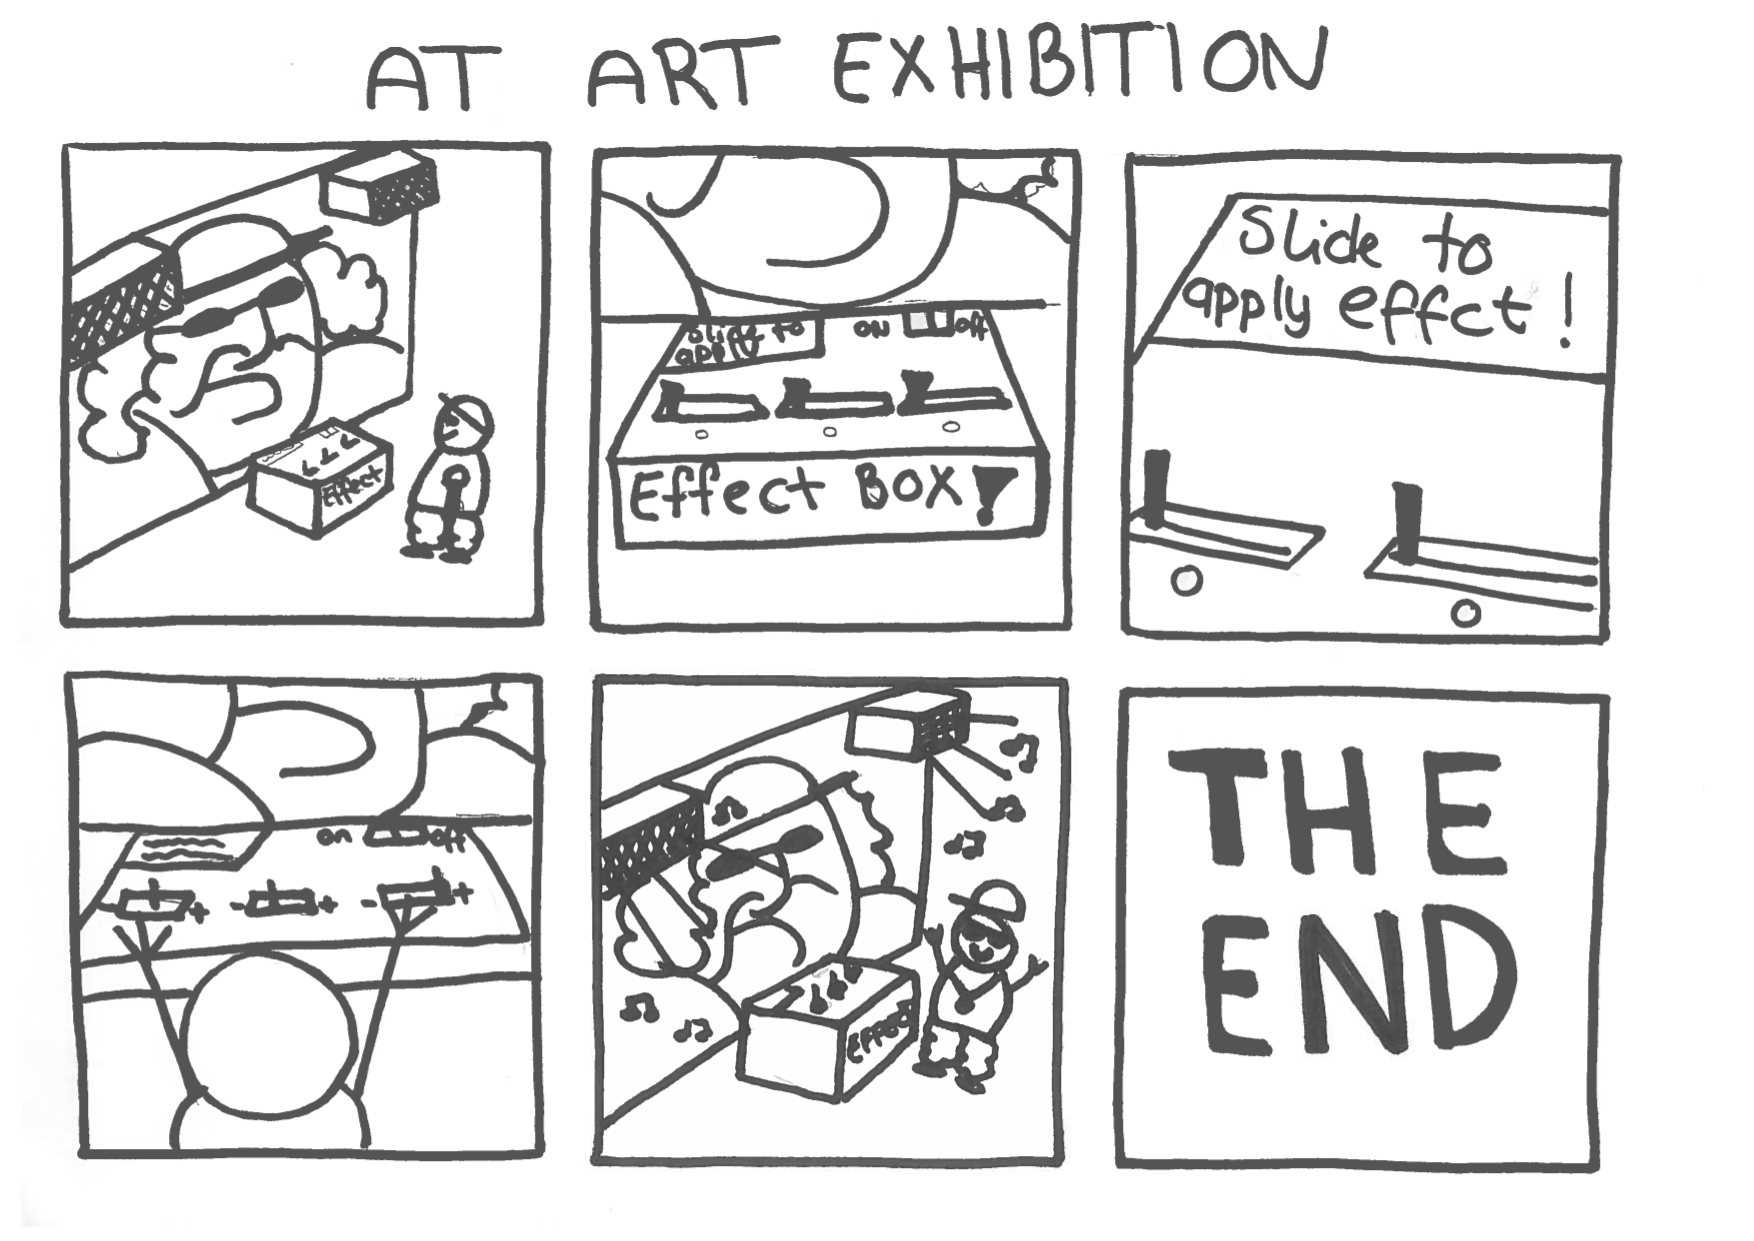
\includegraphics[width=1\textwidth]{Flowdiagram}
<<<<<<< HEAD
\caption{\label{fig:Flowdiagram} A narrative story board of the finish product, in context use.}
=======
\caption{\label{fig:Flowdiagram} A narrative story board of the finish product used in context.}
>>>>>>> origin/master
\end{figure}

\section{Final Prototype}\label{sec:finaldesign final}
The design team elaborated on the earlier designs sketches and with the feedback from the users design tests a final design was made. From Section \ref{sec:lowfitest} it was determined to remove the on and off button as well as giving the user the possibility to switch between the different states in order to avoid confusion and to obtain a more simplistic design. Since the button that decided which slider was active was removed, all three sliders are constantly active. It was also decided to use three sliders to get three different effects, all based on the choices made in the initial brainstorm from Section \ref{sec:initialbrainstorm}. The final design can be seen on Figure \ref{fig:finaldesignsketch3grey}.

\begin{figure}[!h] 
\centering
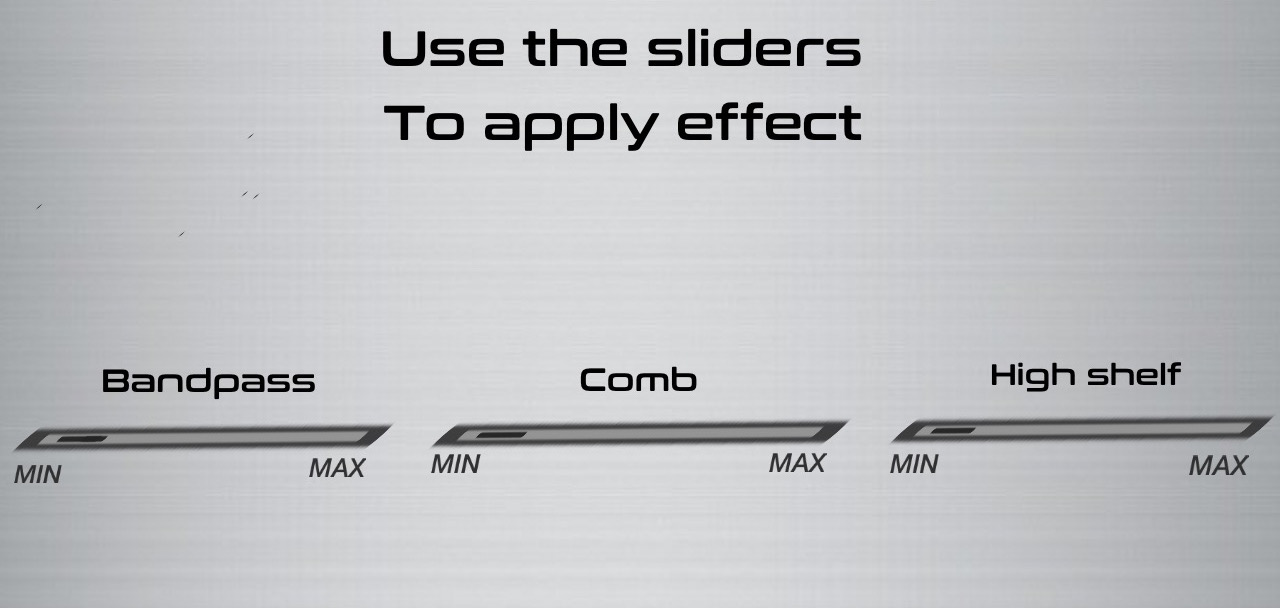
\includegraphics[width=1\textwidth]{Finaldesignfinal}
\caption{\label{fig:finaldesignsketch3grey} The sketch of the final interface design.}
\end{figure}  








